\documentclass[11pt]{article}
\usepackage{url}
\usepackage{graphicx}
\usepackage{pdfpages}
\usepackage{amsmath}%
\usepackage{amsfonts}%
\usepackage{amssymb}%
\usepackage{amsthm}%

\hoffset=-.04\textwidth%
\textwidth=1.08\textwidth%
\voffset=-0.03\textheight
\textheight=1.06\textheight
%\voffset=0.5cm%
%\textheight=1.08\textheight%

\newcommand{\C}{\mathbf{C}}%
\newcommand{\F}{\mathbf{F}}%
\newcommand{\Q}{\mathbf{Q}}%
\newcommand{\Qbar}{\overline{\Q}}%
\newcommand{\Z}{\mathbf{Z}}%
\newcommand{\R}{\mathbf{R}}%
\newcommand{\T}{\mathbf{T}}%
\renewcommand{\H}{\mathrm{H}}%

\newcommand{\eps}{\varepsilon}%
\newcommand{\con}{\equiv}%
\newcommand{\isom}{\cong}%
\newcommand{\rhobar}{\overline{\rho}}
\newcommand{\tensor}{\otimes}


% ---- SHA ----
\DeclareFontEncoding{OT2}{}{} % to enable usage of cyrillic fonts
  \newcommand{\textcyr}[1]{%
    {\fontencoding{OT2}\fontfamily{wncyr}\fontseries{m}\fontshape{n}%
     \selectfont #1}}%
\newcommand{\Sha}{{\mbox{\textcyr{Sh}}}}%
\newcommand{\tor}{\mbox{\scriptsize\rm tor}}

\newcommand{\myname}{William Stein}
\newcommand{\phone}{{\sf (206) 419-0925}}
\newcommand{\email}{{\sf wstein@gmail.com}}
\newcommand{\www}{{\sf http://wstein.org}}
\newcommand{\address}{}
\usepackage{fancyhdr,ifthen}
\pagestyle{fancy}
\cfoot{\thepage}  % no footers (in pagestyle fancy)
% running left heading
\lhead{\bfseries\LARGE\em \noindent{}\hspace{-.2em}\myname{}
        \hfill \thisdocument\vspace{-.2ex}\\}
% running right heading
%\newcommand{\spc}{1.31em}
\newcommand{\spc}{1em}

%\rhead{\em {\small{\phone{}}} \hfill $\cdot$\hfill
% \email{} \hfill $\cdot$\hfill \www{}}

\rhead{\em {\small{\phone{}}} \hfill \email{} \hfill \www{}}

\setlength{\headheight}{5ex}
\newcommand{\mainhead}[1]{\begin{center}{\Large \bf #1}\end{center}}
\newcommand{\head}[1]{\vspace{1.5ex}\par\noindent{\large \bf #1}\par\noindent}
\newcommand{\subhead}[1]{\vspace{2ex}\par\noindent{\sl #1}\vspace{1ex}\par\noindent{}}
\newcommand{\ptitle}{\sl}

\newcommand{\hra}{\hookrightarrow}


%%%% Theoremstyles
\theoremstyle{plain}
\newtheorem{theorem}{Theorem}[section]
\newtheorem{proposition}[theorem]{Proposition}
\newtheorem{corollary}[theorem]{Corollary}
\newtheorem{claim}[theorem]{Claim}
\newtheorem{lemma}[theorem]{Lemma}
\newtheorem{conjecture}[theorem]{Conjecture}

\theoremstyle{definition}
\newtheorem{definition}[theorem]{Definition}
\newtheorem{algorithm}[theorem]{Algorithm}
\newtheorem{question}[theorem]{Question}
\newtheorem{problem}[theorem]{Problem}
\newtheorem{goal}[theorem]{Goal}

\theoremstyle{remark}
\newtheorem{remark}[theorem]{Remark}
\newtheorem{remarks}[theorem]{Remarks}
\newtheorem{example}[theorem]{Example}
\newtheorem{exercise}[theorem]{Exercise}

\DeclareMathOperator{\End}{End}%
\DeclareMathOperator{\Tr}{Tr}%
\DeclareMathOperator{\Res}{Res}%
\DeclareMathOperator{\res}{res}%
\DeclareMathOperator{\BSD}{BSD}%
\DeclareMathOperator{\Gal}{Gal}%
\DeclareMathOperator{\GL}{GL}%
\DeclareMathOperator{\Aut}{Aut}%
\DeclareMathOperator{\Reg}{Reg}%
\DeclareMathOperator{\Vis}{Vis}%
\DeclareMathOperator{\Ker}{Ker}%
\DeclareMathOperator{\Coker}{Coker}%
\DeclareMathOperator{\Sel}{Sel}%
\DeclareMathOperator{\ord}{ord}%
\DeclareMathOperator{\new}{new}%
\DeclareMathOperator{\an}{an}%


\newcommand{\thisdocument}{RRF: Proposed Research}

\begin{document}
\section{Introduction and Rationale}

%[[Provide brief critical review of the pertinent literature, theoretical
%background, and justification for the proposed research. Describe any
%results already achieved, including publications.]]

Most of the PI's published research work is in number theory, which is
an area of pure mathematics.  The PI embarked on a new and risky path
at Harvard in 2005, when he started the Sage mathematical software
project, which has grown substantially since he was recruited by UW in
2006.  There are now around 500 Sage developers, over 10,000 downloads
of Sage per month, and over 55,000 unique visitors each month to the
\url{http://sagemath.org} website.  Sage is a very large free
self-contained program for doing sophisticated mathematics, which you
can download and run on your computer.  It incorporates nearly 100
other programs, and already has interfaces to all other popular math
software systems.  The goal of the Sage project is to create a viable
free open source alternative to the commercial systems Maple,
Mathematica, Matlab and Magma.  The PI has published three articles
about Sage, which are listed in the citations document.

The Sage notebook, whose development was partly supported by the RRF
program in 2009, is the primary user interface to Sage.  It was
designed mainly for use by a relatively small number of people, but
there is a public free version that anybody can freely start using at
\url{http://sagenb.org}.  Sage is software for doing serious number
crunching, so it is extremely resource intensive.  The notebook runs
on one powerful computer that the PI purchased in {\bf 2008} and it
has around 100,000 user accounts!  There are usually well over 50
people attempting to use \url{http://sagenb.org} at any given time.

\begin{center}
\begin{figure}[ht]
\hfill
\includegraphics[height=0.28\textheight]{nb2}
\hfill
\includegraphics[height=0.28\textheight]{nb1}
\hfill
\mbox{}
\caption{Screenshots Showing the Sage Notebook\label{fig:sagenb}}
\end{figure}
\end{center}

\noindent{}{\bf Goal:} {\em Create a web application (based on Sage)
  called Salvus, which is designed from the start to be secure, highly
  available, horizontally scalable and able to robustly handle up to
  10,000 simultaneous users.  Provide both free and non-free accounts,
  with revenue from the non-free subscriptions supporting maintenance
  and purchase of hardware, and the development of Sage.}

Instead of teachers and researchers having to pay to buy expensive
commercial mathematical software and install it on their computers, or
be frustrated with the current Sage notebook, Salvus would provide
them the option to {\em reliably} and efficiently use Sage over the
web and confidently get their students to use it.  At many
institutions, purchasing computer software---especially mathematical
software---is a significant burden, and Sage has helped address this
problem, but the burden of installing, mainting, and upgrading Sage
remains, and the Sage notebook hasn't solved that problem because it
is too slow and unreliable.  This project has the potential to have a
profound impact on education at all levels.

There are several web-based software development environments, e.g.,
\url{https://c9.io/}, which have some similarities to what we plan to
implement with Salvus.  However, Salvus is much more focused on
mathematical algorithm, mathematics education (at all levels), and
mathematical research than any existing web applications.

\section{Objectives}
%What is the project designed to accomplish?

The PI has spent much of Summer 2012 on the foundations of Salvus, and
will make a limited-functionality version available by the end of
September 2012 (see \url{https://salv.us}).  He intends to have a version up and running with
comparable functionality to the existing Sage Notebook by March 2012,
and build a core subscriber base of at least 2500 users by August
2013; work during Winter 2013 is being funded by the remainder of his
startup money, and during some of Summer 2013 by an NSF grant.  This
RRF would allow the PI to work fulltime straight through until late
December 2013 on the next stage of the Salvus project. The specific
goals for the second stage of development will address some
significant {\em functionality} that is completely missing from the
current Sage Notebook and Salvus.

\begin{enumerate}
\item Market an enterprise version of Salvus that customers can
  install on an internal secure network on their own hardware.
\item Greatly improve support for using software other than Sage
  through the Salvus interface, including Octave, Scilab, R, Matlab,
  Mathematica, Maple, and Magma. This will help draw in users from the
  sciences.
\item Implement editors for at least the following document types:
  command line, Latex document, Mathcad style free-form document,
  python and sage files, and for fast interactive 2d and 3d graphics
  using modern web standard such as HTML5 canvas and WebGL.
\item Integrate with many popular cloud storage and repository hosting
  services, including Dropbox, Google Drive, Github, Google Code, and
  Bitbucket.
\item Make it possible for people to write and modify the code that
  gets included with Sage entirely using Salvus, so anybody can
  constribute to Sage without having to install Sage.
\end{enumerate}


\section{Procedure}

% With what methods, materials, or tools will the objectives be met?
% If access to a particular location or institution is required for
% research or data collection, state whether permission has been
% obtained.

\subsection{Computer Hardware}
Purchasing access to computers located at multiple datacenters is
critical to this proposal, given the dual goals of high availability
(fully available even when a data center goes down) and scalability
(10,0000 simultaneous users).

\begin{enumerate}
\item {\bf Padelford Hall Server Room:} 4 1U Dell R415's with 64GB RAM
  and 16 3Ghz cores (one time cost of \$10K)
\item {\bf UW Colocation Facility in the tower:} 4 1U Dell R415's with
  64GB RAM and 16 3Ghz cores (one time cost of \$10K; yearly hosting
  cost of \$1200)
\item {\bf Servedby.net cloud computing
  provider}\footnote{Servedby.net is owned and run by a recent UW
  undergraduate}: 16 8GB instances (cost?)
\item {\bf Amazon.com EC2:} 16 m1.large spot instances (one bids on
  them; they are much cheaper than guaranteed instances; they are not
  always available); cost -- around \$10K/year.
\item {\bf Google App Engine:} the PI was awarded \$60K in Google App
  Engine credits, which can only be used to support Salvus during one
  year from the date of first use.
\end{enumerate}

\subsection{Computer Software}
To support fault tolerance, the PI has designed Salvus so that it has
no single (or even double!) points of failure.  The underlying
database is Cassandra (see \url{http://www.datastax.com/}), which is
designed so that it continues to function well even if several nodes
(or even a whole data center) fails.  Cassandra was open sourced by
Facebook, and is now heavily used by Netflix, Disney, and many other
companies.




\section{Time Schedule}
% Provide a schedule showing how the proposed research can be
% accomplished during the desired support period. The support period
% is normally limited to one year. A no-cost extension of up to one
% year may be granted if requested and adequately justified.

The PI intends to work full time for three months (October -- December 2013):

\begin{enumerate}
\item {\bf October, 2013:} Package and test a standalone enterprise
  version of Salvus.  Work with lawyers at C4C to nail down licensing
  and copyright issues. The PI has existing longterm relationships
  with two large potential customers.  Also, work to improve robust
  support for R, Matlab, Magma, etc., which is of interest to such
  customers.
\item {\bf November, 2013:} Improve support for a wide range of
  filetypes, while integrating Salvus with popular cloud storage and
  hosting services.
\item {\bf December, 2013:} Building on support for repository hosting
  from the previous month, make it possible for people to write and
  modify the code that gets included with Sage entirely using Salvus.
  This will indirectly contribute to the ultimate goal of improving
  the core capabilities of Sage.
\end{enumerate}


\section{Need for RRF Support}
% What other efforts have been made to find support for the project?
% How could the results of the work lead to further outside funding or
% commercial applications? How does this project address the mission
% of the Royalty Research Fund? For RRF Scholar applicants, provide
% documentation of teaching load (quarter, course number, title, and
% credits) in this section.

Though the PI has obtained funding for the Sage project from
Microsoft, Google, the National Science Foundation, prize money,
private donations, and contracts with industry for Sage development,
this has mostly been limited seed money.  The more Sage improves and
grows in quality to equal and exceed the commercial offerings, the
{\em easier} it becomes to obtain further outside funding and for Sage
to be useful in potentially thousands of educational and commercial
applications.

The goals of the current proposal are to greatly enhance Sage's level
of {\em robust availability} and provide a sustainable UW-based
revenue stream to support Sage development.  If successful, this will
have a huge and direct impact both on development of Sage and the
community of Sage users.  This project thus directly addresses the
mission of the Royalty Research Fund by providing a unique opportunity
to increase the PI's competitiveness for subsequent funding via
individual user and site-wide subscriptions to Salvus.

The last RRF that the PI received in 2009 made Sage attractive to the
{\em educational market}, which was a huge area of potential funding
that Sage had not had success in yet.  After that RRF, the Sage
project (and the PI) received a substantial CCLI Type 2 grant (see
\url{http://utmost.aimath.org/}) from the educational part of NSF.
Similarly, supporting the current proposal is likely to expand the
potential funding options for Sage dramatically, by very efficiently
providing a new key service that is in high demand, but nobody
currently makes available.

\subsection{RRF Scholar Application: documentation of teaching load}
The standard teaching load is about 4.5 quarter courses per year.  The
PI is requesting a buyout for 2 Calculus courses (MATH 124: {\em
  Calculus with Analytic Geometry I}, 5 credits, or similar), which he
would likely teach if not supported by an RRF.

\subsection{C4C Letter of Support}\label{sec:letter}
Finally, we close this proposal with a letter of support from the UW
Center for Commercialization, which helps explain how the results of
this work could lead to further funding.

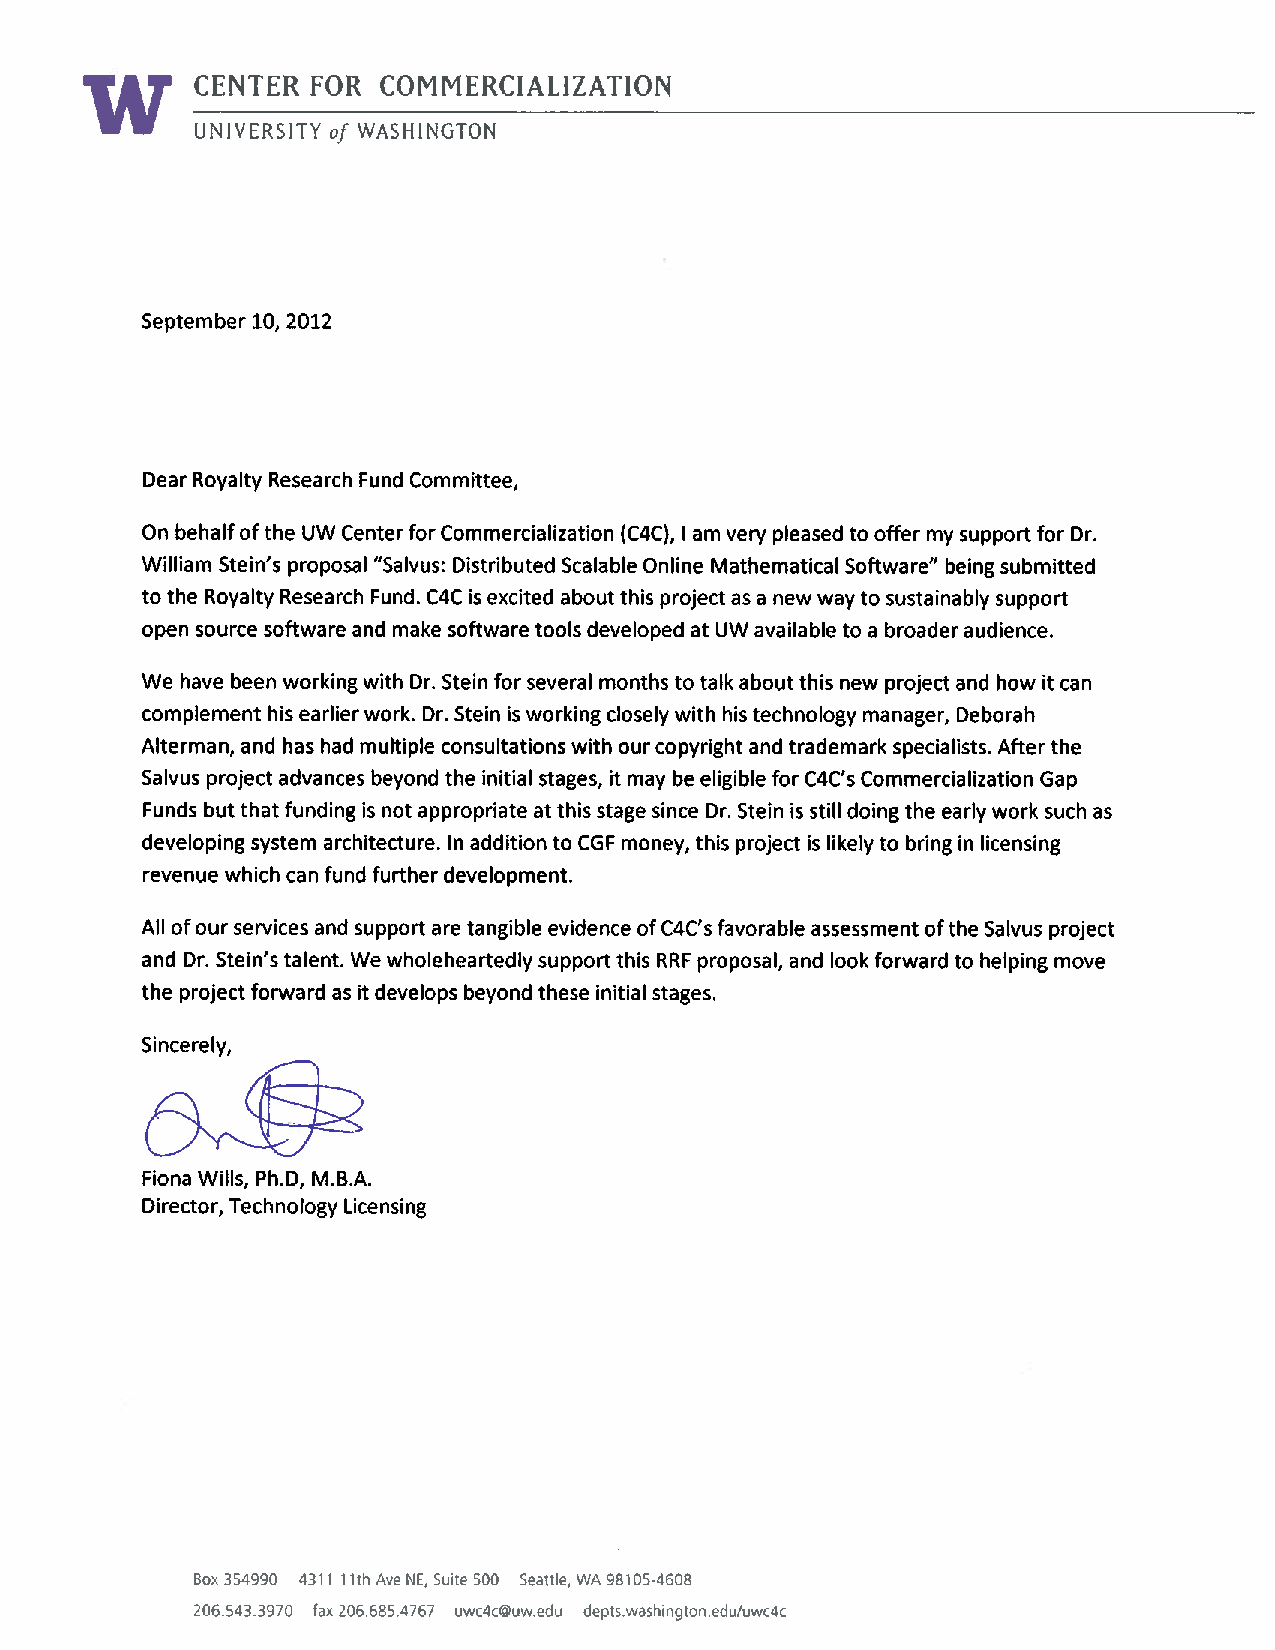
\includepdf[pages=-]{letter_from_c4c}

\end{document}
